\documentclass[18 pt]{beamer}
\usetheme{Madrid}
% \usefonttheme{professionalfonts}
\usefonttheme{structurebold}
\usecolortheme{rose}
\setbeamerfont{title}{size=\LARGE, series=\bfseries}
% \setbeamerfont{subtitle}{size=\large}
% \setbeamerfont{author}{size=\large}
% \setbeamerfont{date}{size=\large}
% \setbeamerfont{frametitle}{size=\Large, series=\bfseries}
% \setbeamerfont{framesubtitle}{size=\large}
% \setbeamerfont{normal text}{size=\huge}
\usepackage{enumitem}
\setlist[enumerate]{label=\arabic*)., leftmargin=*,itemsep=30pt}
\setbeamerfont{enumerate item}{size=\LARGE}

\usepackage{amsmath}
\usepackage{amssymb}
\usepackage{listings}
\usepackage{booktabs}
\usepackage{multirow}
\usepackage{multirow}
\usepackage{lmodern}
\usepackage{xcolor}
\usepackage{float}
\lstset{
  language=Python,  %代码语言使用的是matlab
  % frame=shadowbox, %把代码用带有阴影的框圈起来
  rulesepcolor=\color{red!20!green!20!blue!20},%代码块边框为淡青色
  keywordstyle=\color{blue!90}\bfseries, %代码关键字的颜色为蓝色,粗体
  commentstyle=\color{red!10!green!70}\textit,    % 设置代码注释的颜色
  basicstyle=\footnotesize,
  showstringspaces=true,%不显示代码字符串中间的空格标记
  % numbers=left, % 显示行号
  % numberstyle=8pt,    % 行号字体
  % numberstyle=\color{green},
  stringstyle=\rmfamily\slshape\color[RGB]{128,0,0}, % 代码字符串的特殊格式
  breaklines=true, %对过长的代码自动换行
  extendedchars=false,  %解决代码跨页时,章节标题,页眉等汉字不显示的问题
  escapeinside=``,%代码中出现中文必须加上,否则报错
  texcl=true}

\lstset{breaklines}%自动将长的代码行换行排版

\lstset{extendedchars=false}%解决代码跨页时,章节标题,页眉等汉字不显示的问题

\usepackage{textcomp}
% \usepackage[margin=1in]{geometry}
\usepackage{pythonhighlight}
% \usepackage{minted}
\usepackage[backend=bibtex]{biblatex}
%\usepackage[style=authortitle,backend=biber]{biblatex}
\addbibresource{ResearchRabbit_Export_2022_10_20.bib}

\usepackage{algorithm}
\usepackage{algorithmic}
\renewcommand{\algorithmicrequire}{\textbf{Input:}}
\renewcommand{\algorithmicensure}{\textbf{Output:}}

\AtBeginSection[]{
  \begin{frame}
  \frametitle{Outline}
  \tableofcontents[currentsection]
  \end{frame}
}
\setbeamertemplate{section in toc}{\inserttocsectionnumber.~\inserttocsection}
\setbeamertemplate{subsection in toc}[ball unnumbered]
\setbeamertemplate{subsubsection in toc}[square unnumbered]


\title{Netural Atom Quantum Computation introduction}
\author[Gcc]{Dingchao Gao}
\institute[ISCAS]{Institute of Software Chinese Academy of Sciences}

\setbeamertemplate{footline}[frame number]
\begin{document}

\begin{frame}[plain]
  \titlepage
\end{frame}
\begin{frame}{main reference}
  \begin{enumerate}
    \item Henriet, Loic, Lucas Beguin, Adrien Signoles, Thierry Lahaye, Antoine Browaeys, Georges-Olivier Reymond, and Christophe Jurczak. \textbf{Quantum Computing with Neutral Atoms}. Quantum 4 (21 September 2020): 327. \url{https://doi.org/10.22331/q-2020-09-21-327}.
    \item Bluvstein, Dolev, Harry Levine, Giulia Semeghini, Tout T. Wang, Sepehr Ebadi, Marcin Kalinowski, Alexander Keesling, et al. \textbf{A Quantum Processor Based on Coherent Transport of Entangled Atom Arrays}. Nature 604, no. 7906 (21 April 2022): 451–56. \url{https://doi.org/10.1038/s41586-022-04592-6}.
  \end{enumerate}
\end{frame}
\section{principle}
% \begin{frame}
%   \frametitle{important principle}
%   \begin{enumerate}
%     \item Pauli exclusion principle
%     \item Aufbau principle
%     \footcite{https://en.wikipedia.org/wiki/Aufbau_principle}
%   \end{enumerate}
% \end{frame}
% some basic
% atom 
\subsection{control}
\begin{frame}{optical tweezers}
  \begin{columns} % The "T" option aligns the columns' content at the top

    \begin{column}{.5\textwidth} % Left column, 50% of the text width
    \begin{enumerate}[label=\arabic*., leftmargin=*, itemsep=30pt] % Customize enumerate
        \item First item
        \item Second item
        \item Third item
    \end{enumerate}
    \end{column}
    
    \begin{column}{.5\textwidth} % Right column, 50% of the text width
    \begin{figure}
      \centering
    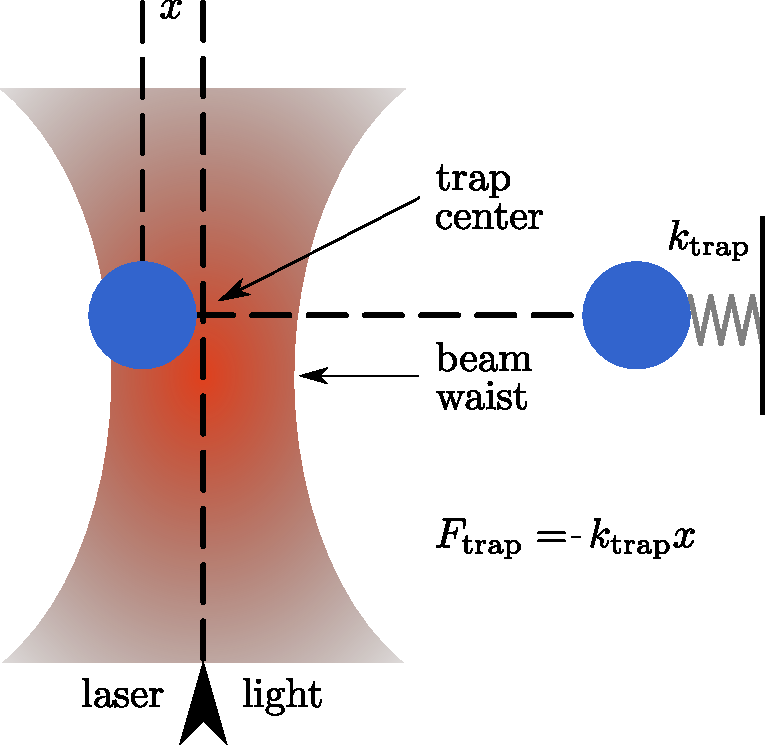
\includegraphics[width=\textwidth]{Optical_trap_prinple} % Adjust the path and image name
    \caption{Figure Caption}
    \end{figure}
    \end{column}
    
  \end{columns}
\end{frame}
\begin{frame}{histroy}
  
\end{frame}
\begin{frame}{optical lattice}
  
\end{frame}
\begin{frame}{work flow}
% rearrange
% AOD
% LCSLM
\end{frame}

% Hamilition
\subsection{operation}
\begin{frame}{readout}
  % a example figure here
\end{frame}
\begin{frame}{single-qubit gate}
  
\end{frame}
\begin{frame}{multi-qubit gate}
\end{frame}
\begin{frame}{Hamilition operation}
\end{frame}
\begin{frame}{summarize}
  % befit of atom
  % scale difficult
  % error source
\end{frame}
\section{device}
\begin{frame}{breakthrough}
  % three different
\end{frame}
\section{computation}
\subsection{compilition}
\begin{frame}{set up}
\end{frame}
\subsection{eror correction}
\section*{end}
\begin{frame}{discussion}
\end{frame}
\end{document}